\documentclass[11pt]{article}

\usepackage{amsmath,amsthm}
\usepackage{hyperref}
\usepackage{graphicx}
\usepackage{caption,subcaption}

\numberwithin{equation}{section}

\theoremstyle{definition}
\newtheorem{theorem}{Theorem}[section]
\newtheorem{remark}[theorem]{Remark}

\usepackage{authblk}

\title{Periodic Traveling Waves in an Integro-Difference Equation With a Nonmonotone Growth Function and Strong Allee Effect}

\author{Michael Nestor, Bingtuan Li
\thanks{M. Nestor's email is \href{mailto:mdnest01@gmail.com}{mdnest01@gmail.com}. B. Li was partially supported by the National Science Foundation under Grant DMS-1515875 and Grant DMS-1951482.}}

\affil{Department of Mathematics, University of Louisville, \newline Louisville, KY 40292.}


\begin{document}


\maketitle


\begin{abstract}
We analytically establish the existence of a periodic traveling wave for an integro-difference equation with a growth function exhibiting a period two cycle and a strong Allee effect. We also prove the convergence of solutions with compactly supported initial data to translations of the traveling wave under appropriate conditions. 
\end{abstract}


{\bf Key words:} Integro-difference equation, period two cycle, Allee effect, periodic traveling wave.
\newline

{\bf AMS Subject Classification:} 92D40, 92D25.


\section{Introduction}

Integro-difference equations are of great interest in the studies of invasions of populations with discrete generations and separate growth and dispersal stages. They have been used to predict changes in gene frequency \cite{lui82a, lui82b, lui83, slatkin, w78}, and applied to ecological problems~\cite{hh, ks, kot89, kot92, kotbook, lut, nkl,otto}. Previous rigrous studies on integro-difference equations have assumed that the growth function is nondecreasing~\cite{w78, wein82}, or  is nonmonotone without strong Allee effect~\cite{lui83, wang}. The results show existence of constant spreading speeds and travelng waves with fixed shapes and speeds.   Sullivan et al. ~\cite{pnas} demonstrated numerically  that an integro-difference equation with a nonmonotone growth function exhibiting  a strong Allee effect can generate traveling waves with fluctuating speeds. In this paper we analytically prove the existence of periodic traveling waves with a periodic speed for such an equation with a specific growth function and dispersal kernel.


We consider the following integro-difference equation
\begin{align}\label{q}
u_{n+1}(x)\;=\;Q[u_n](x)\;:=(k*(g\circ u_n))(x)\;=\,\int^{\infty}_{-\infty}k(x-y)\,g\big(u_n(y)\big)\,\mathrm{d}y,
\end{align}
where 
\begin{equation} \label{g}
g(u) = \begin{cases}
0, & \text{if } 0 \leq u < a, \\
n_2, & \text{if } a \leq u < b, \\
n_1, & \text{if } u \geq b,
\end{cases}
\end{equation}
with 
$0<a<n_1<b<n_2$,
and
\begin{equation} \label{k}
k(x) = \begin{cases}
\frac{1}{2\alpha}, & \text{if } |x| \leq \alpha, \\
0, & \text{otherwise},
\end{cases}
\end{equation}
with $\alpha >0$. $g(u)$ is a piecewise constant nonmonotone growth function exhibiting a strong Allee effect~\cite{all}. Specifically, it has a stable fixed point at zero and a stable period two cycle $(n_1,n_2)$ with $a$ the Allee threshold value. The graph of $g(u)$ with $a=0.33,b=0.75,n_1=0.5,n_1=1.0$ is depicted in Figure \ref{fig:g}.
\begin{figure}
\begin{center}
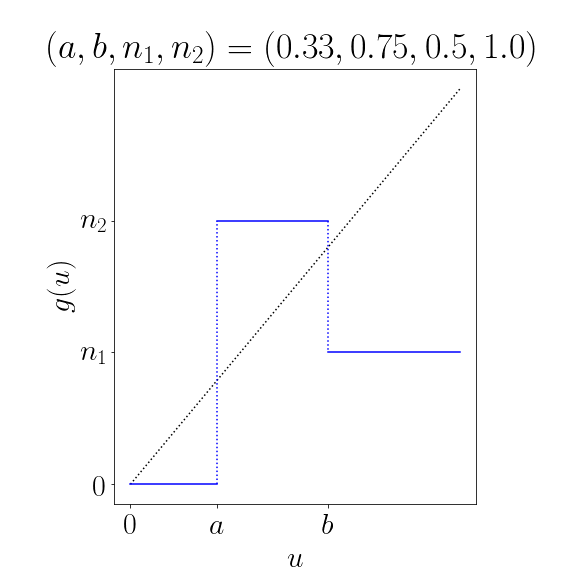
\includegraphics[width=0.5\textwidth]{fig1}
\end{center}
\caption{The growth function $g(u)$ with $(a,b,n_1,n_2)=(0.33,0.75,0.5,1.0)$.}
\label{fig:g}
\end{figure}
$k(x)$ is a uniform distribution. Piecewise constant growth functions and uniform distributions have been used in the studies of integro-difference equations; see for example~\cite{kot1, lut,otto,  pnas}. We rigorously construct periodic traveling waves with periodic speeds for (\ref{q}). To the best of our knowledge, this is the first time that traveling waves with oscillating speeds have been analytically established  for scalar spatiotemporal equations with constant parameters. We also show the convergence of solutions with compactly supported initial data to translations of the traveling wave under appropriate conditions. Equation (\ref{q}) may be viewed as a symbolic model for integro-difference equations with a growth function exhibiting a strong Allee effect and a period two cycle. The results obtained this paper provide important insights into integro-difference equations with general growth functions and dispersal kernels. 


\section{Periodic traveling waves}

Let $x_0 = \alpha \left(1-\frac{2b}{n_2}\right)$ and $c_1 = \alpha \left(1- \frac{2a}{n_2}\right)$.
Define 
\begin{equation}  \label{w1}
\begin{aligned}
w_1(x) 
= \begin{cases}
n_2, & x \in (-\infty, -\alpha), \\
\frac{n_2}{2} - \frac{n_2}{2\alpha}x, & x \in [-\alpha, \alpha] ,\\
0, & x \in (\alpha, \infty),
\end{cases}
\end{aligned} \end{equation}
and 
\begin{equation} \label{w2}
\begin{aligned}
w_2(x) 
= \begin{cases}
n_1,
& x \in (-\infty, x_0-\alpha), \\
\frac{n_2-n_1}{2\alpha}(x - (x_0 - \alpha))+n_1,
& x \in [x_0 - \alpha, 
 c_1- \alpha), \\
-\frac{n_1}{2\alpha}(x-(x_0+\alpha))+b-a,
& x \in [c_1 - \alpha, x_0 + \alpha), \\
-\frac{n_2}{2\alpha} (x - (c_1 + \alpha)),
& x \in [x_0 + \alpha, c_1 + \alpha], \\
0,
& x \in (c_1+\alpha,\infty).
\end{cases}
\end{aligned} \end{equation}


\begin{figure*} \label{fig2}
    \centering
    \begin{subfigure}[t]{0.5\textwidth}
        \centering
        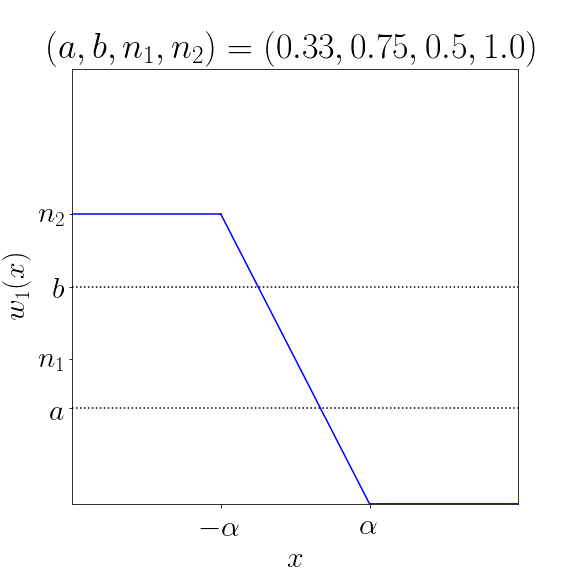
\includegraphics[scale=0.25]{fig2a}
        \caption{$w_1(x)$}
    \end{subfigure}%
    ~ 
    \begin{subfigure}[t]{0.5\textwidth}
        \centering
        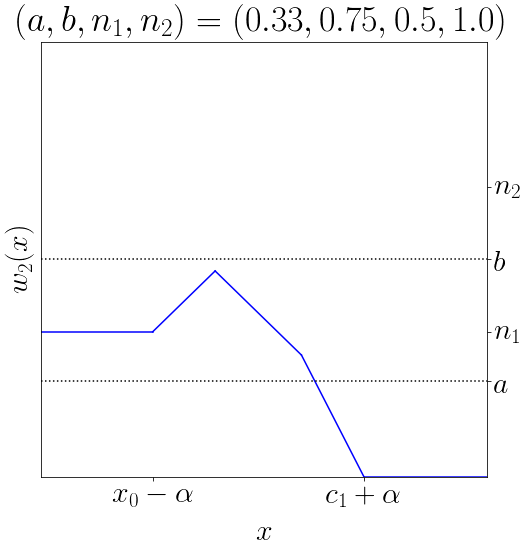
\includegraphics[scale=0.25]{fig2b}
        \caption{$w_2(x)$}
    \end{subfigure}
    \caption{Profiles of $w_1(x)$ and $w_2(x)$ with $(a,b,n_1,n_2)=(0.33,0.75,0.5,1.0)$.}
    \label{fig:w1andw2}
\end{figure*}

Clearly $w_1(x)$ is non-increasing while $w_2(x)$ is nonmonotonic. The graphs of $w_1(x)$ and $w_2(x)$ with specific parameter values are given in Figure \ref{fig:w1andw2}.



\begin{theorem}\label{thm1}
Let
\begin{equation} \label{h1}
0<a<n_1<b<n_2, \  \   \frac{n_2}{n_1} < \frac{b-a}{n_1-a}.
\end{equation}
Then 
$$w_2(x)=Q[w_1](x),  \   \   w_1(x-2c^*)=Q[w_2](x),$$
 with 
\begin{equation} \label{c}
c^* = \begin{cases}
\alpha \left( 1 - \frac{2}{n_2}a \right), & \text{if } a \leq b/2, \\
\alpha \left( 1  + \frac{b - 2a}{n_1} - \frac{b}{n_2} \right), & \text{if }a > b/2.
\end{cases}
\end{equation}
\end{theorem}


\begin{proof} $w_1(x)$ can be written as
$$
    w_1(x) = n_2 (1-K(x)),
$$
where $K(x)$ is the cumulative density function $K(x) = \int_{-\infty}^{x} k(y)$. Then $w_1(x)$ is decreasing on $(-\alpha,\alpha)$, and satisfies $0\leq w_1(x)<a$ for $x\in(c_1,\infty)$, $a\leq w_1(x)<b$ for $x\in[x_0,c_1]$, and $w_1(x)\geq b$ for $x\in(-\infty,x_0)$. Thus, $g(w_1(x))$ is given by
$$
g( w_1(x)) = \begin{cases}
n_1, & x \in (-\infty, x_0), \\
n_2, & x \in [x_0, c_1], \\ 
0, & x \in (c_1, \infty). \end{cases}.
$$
Applying convolution with $k(x)$:
$$ \begin{aligned}
    Q[w_1](x) &= (k*(g\circ w_1))(x) \\&= (n_2-n_1) K(x-x_0) - n_2 K(x-c_1).
\end{aligned} $$
Computing the right hand side yields $\eqref{w2}$, thus $Q[w_1]=w_2$.

To compute $Q[w_2]$, observe that $w_2$ has a global maximum at $c_1-\alpha$, and that the last inequality in $\eqref{h1}$ is equivalent to $w_2(c_1-\alpha)<b$. Hence, $w_2(x)<b$ for all $x$. Note that $w_2(x)$ decreases from its maximum at $c_1-\alpha$ to zero on the interval $[c_1-\alpha,c_1+\alpha]$, so there is a unique point $\xi$ in this interval such that $w_2(\xi)=a$. Therefore,
$$
g(w_2(x)) = \begin{cases}
n_2, & x \in (-\infty,\xi], \\
0, & x \in (0,\infty).
\end{cases}
$$
and
$$ \begin{aligned}
Q[w_2](x)
&= n_2 (1-K(x-\xi)) \\
&= w_1(x-\xi).
\end{aligned} $$

By defining $c^*=\xi/2$, we have $w_1(x-2c^*)=Q[w_2](x)$. Thus, $w_1(x)$ and $w_2(x)$ form a period two traveling wave with average speed $c^*$.

The value of $c^*$ can be computed as the unique solution to $w_2(2c^*)=a$, or equivalently $c^*=\frac{1}{2}w_2^{-1}(a)$. Observe that $w_2(x_0+\alpha)-a=b-2a$, so there are two cases. If $a\leq b/2$ then $\xi\in[x_0+\alpha,c_1+\alpha]$, and $c^*$ is given by $c^*=\frac{1}{2}\ell_1^{-1}(a)=\alpha \left( 1 - \frac{2}{n_2}a \right)$ where
$$ \ell_1(x)=-\frac{n_2}{2\alpha} (x - (c_1 + \alpha)).$$
Otherwise, if $a>b/2$, then $\xi\in[c_1-\alpha,x_0+\alpha)$ and $c^*=\frac{1}{2}\ell_2^{-1}(a)=\alpha \left( 1  + \frac{b - 2a}{n_1} - \frac{b}{n_2} \right)$ where
$$ \ell_2(x)=-\frac{n_1}{2\alpha}(x-(x_0+\alpha))+b-a.$$
The proof is complete.
\end{proof}


\begin{remark}
$w_1(x)$ is positive for $x<\alpha$ and zero for $x\geq\alpha$, and $w_2(x)$ is positive for $x<c_1+\alpha$ and zero for $x\geq c_1+\alpha$.  $Q[w_1](x)=w_2(x)$ shows that the wave front point travels a distance $c_1$, and $Q[w_1](x)=w_1(x-2c^*)$ indicates that the wave front point travels a distance $c_2=2c^*-c_1$. This theorem shows that $\eqref{q}$ has a traveling wave with wave profiles $w_1(x)$ and $w_2(x)$, intermediate wave speeds $c_1$ and $c_2$,  and average wave speed  $c^*$.  It is easily seen that $c_1=c_2$ if $a \leq b/2$, and $c_1-c_2=2\alpha (b-2a)(\frac{1}{n_2}-\frac{1}{n_1})\not=0$ if $a>b/2$. So for $a>b/2$, the traveling wave is periodic with two different intermediate wave speeds. This behavior is illustrated with two difference choices of parameters in Figure \ref{fig:wavespeed}.
\end{remark}

\begin{remark}
The traveling wave is advancing if $c^*>0$ and receding if $c^*<0$. The sign of the wave speed can be written in two cases:
\begin{equation}
\text{sign}(c^*) = \text{sign}\left(n_2 - 2a\right), \text{ if } a \leq b/2, \end{equation}
and
\begin{equation}
\text{sign}(c^*) =
\text{sign}\left(\frac{n_1}{n_2} - \frac{2a-b}{n_2-b}\right),  \text{ if } a > b/2. 
\end{equation}
\end{remark}

\begin{remark}
$w_1(-x)$ and $w_2(-x)$ are profiles of a traveling wave moving leftward at 
 intermediate wave speeds $c_1$ and $c_2$, and average wave speed  $c^*$. This is due to the fact that $Q$ is symmetric and translation invariant.
\end{remark}


\begin{figure*}
    \centering
    \begin{subfigure}[t]{0.5\textwidth}
        \centering
        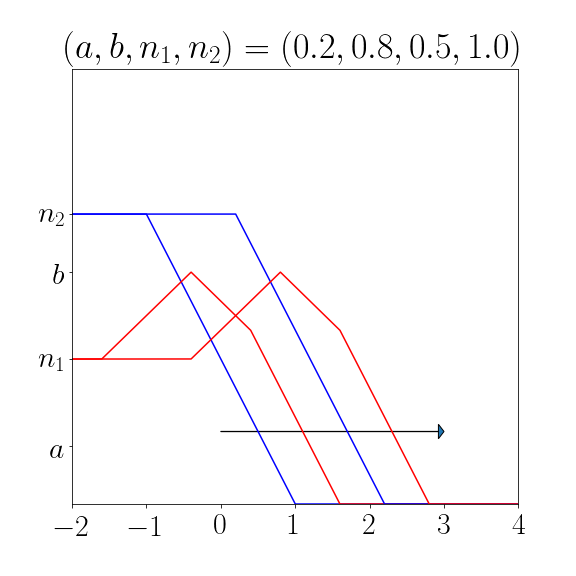
\includegraphics[scale=0.25]{fig3a}
        \caption{Constant wave speed, \newline $(a,b,n_1,n_2)=(0.2,0.8,0.5,1.0)$.}
    \end{subfigure}%
    ~ 
    \begin{subfigure}[t]{0.5\textwidth}
        \centering
        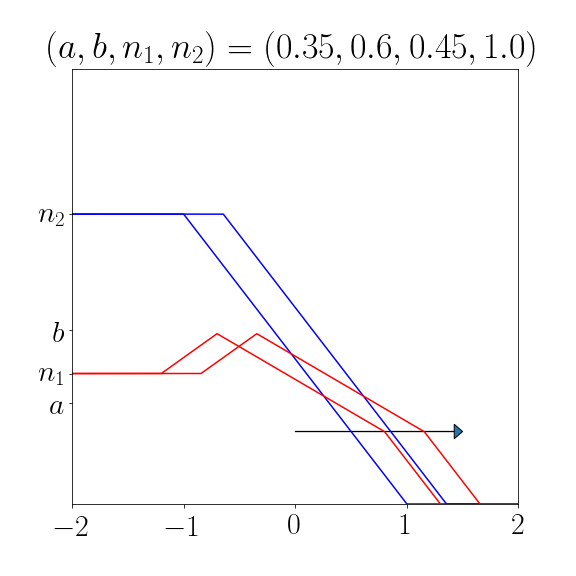
\includegraphics[scale=0.25]{fig3b}
        \caption{Oscillating wave speed, \newline $(a,b,n_1,n_2)=(0.35,0.6,0.45,1.0)$.}
    \end{subfigure}
    \caption{Traveling wave behavior of $w_1(x)$ and $w_2(x)$.}
    \label{fig:wavespeed}
\end{figure*}


The regions in the parameter space where oscillating spreading speed exists can be determined as follows: for any fixed choice of $(n_1,n_2)$, with $0<n_1<n_2$, let $R$ be the set of pairs $(a,b)\in\mathbf R^2$ such that the hypothesis of Theorem 2.1 holds. Then $R$ is a triangle in the $a$-$b$ plane with endpoints at $(0,n_2)$, $(n_1,n_1)$, and $(n_1,n_2)$, depicted in Figure \ref{fig:phaseportrait}. The line $b=2a$ partitions $R$ into two non-empty sets $R_1=\{(a,b)\in R:a\leq b/2\}$ and $R_2=\{(a,b)\in R:a> b/2\}$ such that the traveling has constant speed if $(a,b)\in R_1$ and oscillating speed if $(a,b)\in R_2$.


\begin{figure}
\begin{center}
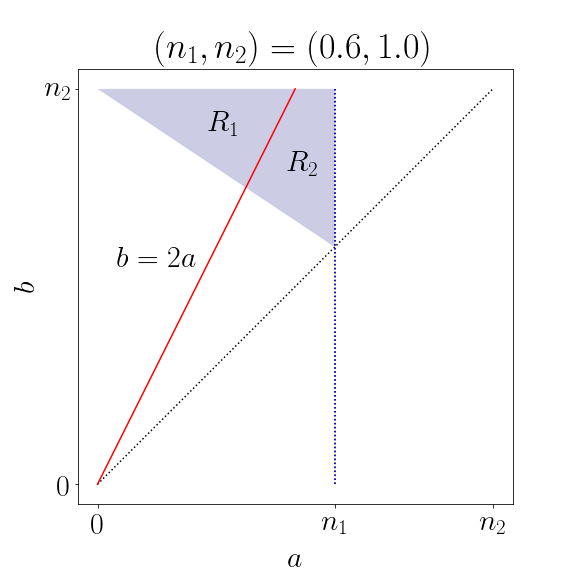
\includegraphics[width=0.5\textwidth]{fig4}
\end{center}
\caption{The shaded region $R$ indicates all pairs $(a,b)$ such that the condition in Theorem 2.1 holds for $(n_1,n_2)=(0.6,1.0)$, and the line $b=2a$ is drawn in red. The region $R_1$ contains all pairs $(a,b)$ such that the traveling wave has constant speed, and $R_2$ contains all pairs such that the traveling wave has oscillating speed.}
\label{fig:phaseportrait}
\end{figure}


The next theorem concerns convergence of solutions with compactly supported initial data to translations of the traveling wave. Let
\begin{equation}
r_0 = \max\left\{2\alpha,2\alpha-x_0\right\}.
\end{equation}
\begin{theorem} Assume that the hypothesis of Theorem~\ref{thm1} holds and $c^*\geq0$.  Let $a\leq  u_0(x)<b $ on $[L-r, L+r]$ with $r\geq r_0$ and $L$ a real number, $u_0(x)<a$  for $x\not\in [L-r, L+r]$, and $u_0(x)\equiv 0$ outside a bounded interval.  
Then the solution $u_n$ of $u_{n+1}=Q[u_n]$ is given by
\begin{equation}
u_{2n+1}(x) = \begin{cases}
w_1(x-L-r-2nc^*), & x\in[L,\infty), \\
w_1(-x+L-r-2nc^*), & x\in(-\infty,L),
\end{cases}
\end{equation}
and
\begin{equation}
u_{2n+2}(x) = \begin{cases}
w_2(x-L-r-2nc^*),  & x\in[L,\infty), \\
w_2(-x+L-r-2nc^*), & x\in(-\infty,L).
\end{cases}
\end{equation}
\end{theorem}


\begin{figure*} \label{fig5}
    \centering
    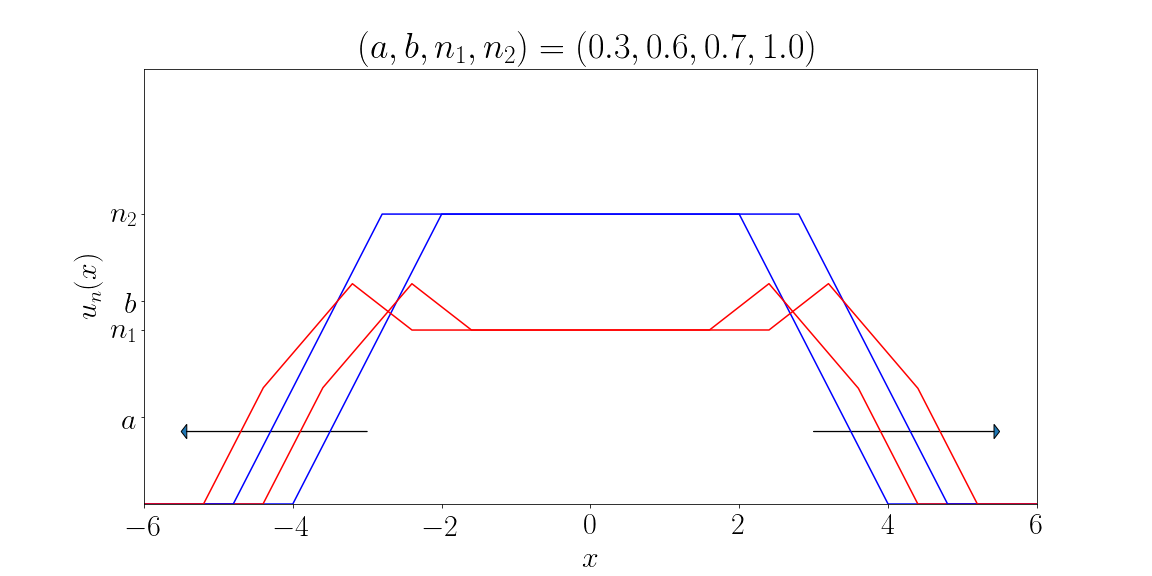
\includegraphics[scale=0.25]{fig5}
    \caption{Speading behavior for bounded initial data with $(a,b,n_1,n_2)=(0.3,0.6,0.7,1.0)$. Shapes of $u_1$ and $u_3$ are labeled in blue, shapes of $u_2$ and $u_4$ in red.}
\label{fig:spread}
\end{figure*}


\begin{proof}
The composition of $g$ with $u_0$ is given by
$$
    g(u_0(x+L)) = \begin{cases}
    n_2, & x \in [-r,r], \\
    0, & x \in(-\infty,-r)\cup(r,\infty).
    \end{cases}
$$
Applying convolution with $k$,
$$ \begin{aligned}
u_1(x+L) &= (k*(g\circ u_0))(x+L) \\
&= n_2 \left( K(x+r)-K(x-r) \right) \\
&= w_1(x-r) - w_1(x+r).
\end{aligned} $$
If $x\geq 0$ and $r\geq \alpha$, then $w_1(x+r)=0$, and hence $u_1(x)=w_1(x-r)$. By the symmetry of $g(u_0(x))$ about the line $x=L$, and the symmetry of the operator $Q$, it follows that $u_1$ is also symmetric about $x=L$, hence
$$ u_1(x+L) = \begin{cases}
w_1(x-r), & x \in [0,\infty), \\
w_1(-x-r), & x \in (-\infty,0).
\end{cases} $$
The support of $u_1$ is $[L-r-\alpha,L+r+\alpha]$. It satisfies $u_1(x+L)=n_2$ for all $x\in[-r+\alpha,r-\alpha]$. Thus $u_1(x+L)=w_1(x-r)$ for all $x\in[-r+\alpha,\infty)$. Applying the operator $Q$, it follows $Q[u_1](x+L)=Q[w_1](x-r)$ for all $x\in[-r+2\alpha,\infty)$. Since $r\geq 2\alpha$, this implies $u_2(x+L)=w_2(x-r)$ for all $x\geq 0$. $Q$ is a symmetric operator, so
$$ u_2(x+L) = \begin{cases}
		w_2(x-r), & x\in[0,\infty), \\
		w_2(-x-r), & x\in(-\infty,0).
\end{cases} $$
$u_2$ has support $[L-r-c_1-\alpha,L+r+c_1+\alpha]$. It satisfies $u_2(x+L)=n_1$ for all $x\in[-r-x_0+\alpha,r+x_0-\alpha]$. Thus $u_2(x+L)=w_2(x-r)$ for all $x\in[-r-x_0+\alpha,\infty)$. Applying the operator $Q$, it follows $Q[u_2](x+L)=Q[w_2](x-r)$ for all $x\in[-r-x_0+2\alpha,\infty)$. Since $r\geq 2\alpha-x_0$ we have $u_2(x+L)=Q[w_2](x-r)$ for all $x\geq 0$. By Theorem 2.1, $u_2(x+L)=w_1(x-r-2c^*)$ for all $x\geq 0$. Since $Q$ is a symmetric operator, we have 
$$ u_3(x+L) = \begin{cases}
		w_1(x-r-2c^*), & x\in[0,\infty), \\
		w_1(-x-r-2c^*), & x\in(-\infty,0).
\end{cases} $$
If $c^*\geq0$, then this process may be repeated inductively, so that
$$
u_{2n+1}(x+L) = \begin{cases}
w_1(x-r-2nc^*), & x\in[0,\infty), \\
w_1(-x-r-2nc^*), & x\in(-\infty,0),
\end{cases} $$
and
$$
u_{2n+2}(x+L) = \begin{cases}
w_2(x-r-2nc^*),  & x\in[0,\infty), \\
w_2(-x-r-2nc^*), & x\in(-\infty,0).
\end{cases} $$
Replacing $x$ by $x-L$, the proof is complete.
\end{proof}

\begin{remark}
This theorem indicates that a solution with proper compactly supported initial data coverges to translations of periodic traveling waves with profiles $w_1(x)$ and $w_2(x)$ in the positive direction and profiles $w_1(-x)$ and $w_2(-x)$ in the negative direction.
\end{remark}



\begin{thebibliography}{9}
\bibitem{all}  W. C. Allee. 1931. Animal Aggregations. A Study on
General Sociology. University of Chicago Press, Chicago, IL.


%\bibitem{htw90} D. P. Hardin, P. Tak$\acute{\mbox{a}}\check{\mbox{c}}$, and G. F. Webb. 1990. Dispersion population %models discrete in time and
%continuous in space. J. Math. Biol. {\bf 28}: 1-20.

\bibitem{hh} A. Hastings and K. Higgins. 1994. Persistence of transients in spatially
structured ecological models. Science {\bf 263}: 1133-1136.

%\bibitem{hz} S.-B. Hsu and X.-Q. Zhao. 2008. Spreading speeds and traveling waves for nonmonotone integrodifference equations. SIAM J. Math. Anal. {\bf} 40: 776–789


\bibitem{ks} M. Kot and W. M. Schaffer. 1986.  Discrete-time growth-dispersal models.
Math. Biosci. {\bf 80}: 109-136.


\bibitem{kot89} M. Kot. 1989. Diffusion-driven period doubling bifurcations.
Biosystems {\bf 22}: 279-287.


\bibitem{kot92} M. Kot. 1992. Discrete-time traveling waves:
Ecological examples. J. Math. Biol. {\bf 30}: 413-436.


\bibitem{kot1} M. Kot, M. A. Lewis, and P. van den Driessche. 1996. Dispersal data and the spread of invading
organisms. Ecology {\bf 77}: 2027-2042.


%\bibitem{kot2} M. Kot, J. Medlock, T. Reluga, and D. B. Walton. 2004. Stochasticity, invasions, and branching random walks. Theor. Popul. Biol. {\bf 66}: 175-184.


%\bibitem{li09} B. Li, M. A. Lewis, and H. F. Weinberger. 2009.  Existence of traveling waves for integral recursions with nonmonotone growth functions. J. Math. Biol. {\bf 58}: 323-338.


\bibitem{kotbook} M. Kot. 2001. Elements of Mathematical Ecology.
Cambridge University Press. Cambridge, United Kingdom.

\bibitem{lui82a} R. Lui. 1982. A nonlinear integral operator arising from a model in population
genetics. I. Monotone initial data. SIAM. J. Math. Anal. {\bf 13}:
913-937.

\bibitem{lui82b} R. Lui. 1982. A nonlinear integral operator arising from a model in population
genetics. II. Initial data with compact support. SIAM. J. Math.
Anal. {\bf 13}: 938-953.

\bibitem{lui83} R. Lui. 1983. Existence and stability of traveling wave solutions of a nonlinear
integral operator. J. Math. Biol. {\bf 16}:199-220.

\bibitem{lut}
F. Lutscher. 2019. Integrodifference Equations in Spatial Ecology.  Springer.


\bibitem{nkl} M. Neubert, M. Kot, and M. A. Lewis. 1995. Dispersal and pattern formation in a
discrete-time predator-prey model. Theor. Pop. Biol. {\bf 48}
: 7-43.

\bibitem{otto} G. Otto. 2017. Non-spreading Solutiona in a Integro-Difference Model Incorporating Allee and Overcompensation Effects. Ph. D thesis, University of Louisville.

\bibitem{slatkin} M. Slatkin. 1973. Gene flow and selection in a cline.
Genetice {\bf 75}: 733-756.



\bibitem{pnas} L. L. Sullivan, B. Li, T. E. X. Miller, M. G. Neubert, and A. K. Shaw. 2017.
Density dependence in demography and dispersal generates fluctuating invasion speeds. Proc. Natl. Acad. Sci. USA {\bf
114}: 5053-5058.


\bibitem{wang} M. H. Wang, M. Kot, and M. G. Neubert. 2002. Integrodifference equations, Allee effects, and
invasions. J. Math. Biol. {\bf 44}: 150-168.

\bibitem{w78} H. F. Weinberger. 1978. Asymptotic behavior of a model in  population genetics,
in Nonlinear Partial Differential Equations  and Applications, ed.
J. M. Chadam. Lecture Notes in Mathematics {\bf 648}: 47-96.
Springer-Verlag, Berlin.

\bibitem{wein82} H. F.  Weinberger. 1982. Long-time beahvior of a class of biological models. SIAM. J.
Math. Anal. {\bf 13}: 353-396.

\end{thebibliography}

\end{document}









\end{document}
